\documentclass{article} % For LaTeX2e
% We will use NIPS submission format
\usepackage{nips13submit_e,times}
% for hyperlinks
\usepackage{hyperref}
\usepackage{placeins}
\usepackage{url}
% For figures
\usepackage{graphicx} 
% math packages
\usepackage{amsmath}
\usepackage{amsfonts}
\usepackage{amsopn}
\usepackage{ifthen}
\usepackage{natbib}
\usepackage{caption}
\usepackage{subcaption}

\usepackage{booktabs}
\newcommand{\ra}[1]{\renewcommand{\arraystretch}{#1}}

\title{Convolutional Neural Networks using separable filters}
\author{
\fontsize{8}{8}\selectfont{Petrescu Viviana}\\
\fontsize{8}{8}\selectfont{EPFL} \\
\fontsize{8}{8}\selectfont{\texttt{viviana.petrescu@epfl.ch}} \\
}

\nipsfinalcopy 

\begin{document}

\maketitle

\begin{abstract}
CNN are the state-of-the-art machine learning techniques which achieved best results on various computer vision tasks ranging from the large scale ImageNet object recognition challenge to segmentation in bio medical imaging.
This technical report presents initial results on using CNN with separable filters for speeding up the testing time.
\end{abstract}

\section{Introduction}
Although proven to be very powerful, CNN are much slower for both training and testing than their counter parts SVM or Random Forests.
In the forward pass, the computational complexity of evaluating one image os size $W\timesH$ with $J$ filters of size $k_{1}\timesk_{2}$ is $O(WHJd_{1}d{2})$. If the 2d filters are decomposed into separable 1d filters of rank $K$, the complexity becomes
 $O(WH(J +d_{1}+d{2})$. Thus, we obtain a speedup if $K<< \frac{Jd_{1}d_{2}}{J +d_{1}+d_{2}}$. 
 
 Although improving training time would be very beneficial since it would allow for more configurations to be tried and larger networks, increasing effort has been put also into speeding up testing time, since training can be done once.
 
 Picture from [..]
 
 The theoretical rank of a 3D tensor $R$ is less or equal with $prod$.
 This means that for 'tall' set of tensors like the ones present in CNNs 
 $J \times k_{1} \times k_{2}$ with $k_{1}\times k_{2}  J$ we should expect the rank
 to be equal with the product of the two kernel dimensions.
 Some inequalities that hold for the theoretical rank are presented below: $\chi \in \mathbb{R}^{I\times J\times K}$. The typical rank is any rank that occurs with probability greater than 0. FFT
 Other common typical ranks:

\section{Speeding up CNN}
 For the sake of completeness, some approaches that were previously tried were on \citep{Jaderberg14b}, which prove speedup for CNNs for 3 different schemes, one of which it is similar with our approach but using a different optimization algorithm for obtaining the separable filters. Other approached would be to heavily employ the GPU and even employ the FGPA, which are harder to program \citep{lecun2010convolutional}
 Talk about current available programming tools
 - Caffee increasingly popular 
 - Theano symbolic based
 - Torch7 
 - mathLib


Talk about CNN with separable filters and with GPU, fgpa etc

\section{Experiments}
\subsection{MNIST}
MNIST consists of a curated set of postal digits images, of size 28x28.
The training set contains 60000 samples, validation 10000 and testing
10000 samples.
The approached of YannLecun[98] and Ciresan[] proved very good performance. The reference Theano model of Theano achieves 0.82 error rates.
\subsubsection{Model 1}
\begin{table}
\centering
\begin{tabular}{@{}rlll@{}}\toprule
Layer & Type & Maps and neurons& Kernel size \\ \midrule
0 & input & 1 map of 28x28 &\\
1& convolutional & 20 maps of 24x24 & 5x5\\
2 & max pooling & 20 maps of 12x12 & 2x2 \\
3 & convolutional & 50 maps of 8x8& 5x5 \\
4 & max pooling & 50 maps of 4x4& 2x2 \\ 
5 & fully conntected& 500 & \\
6 & fully conntected & 2 neurons & \\ \bottomrule
\end{tabular}
\caption{Small CNN for MNIST set}
\end{table}


\begin{figure}[h]
  \centering
  \begin{subfigure}[b]{0.40\textwidth}
   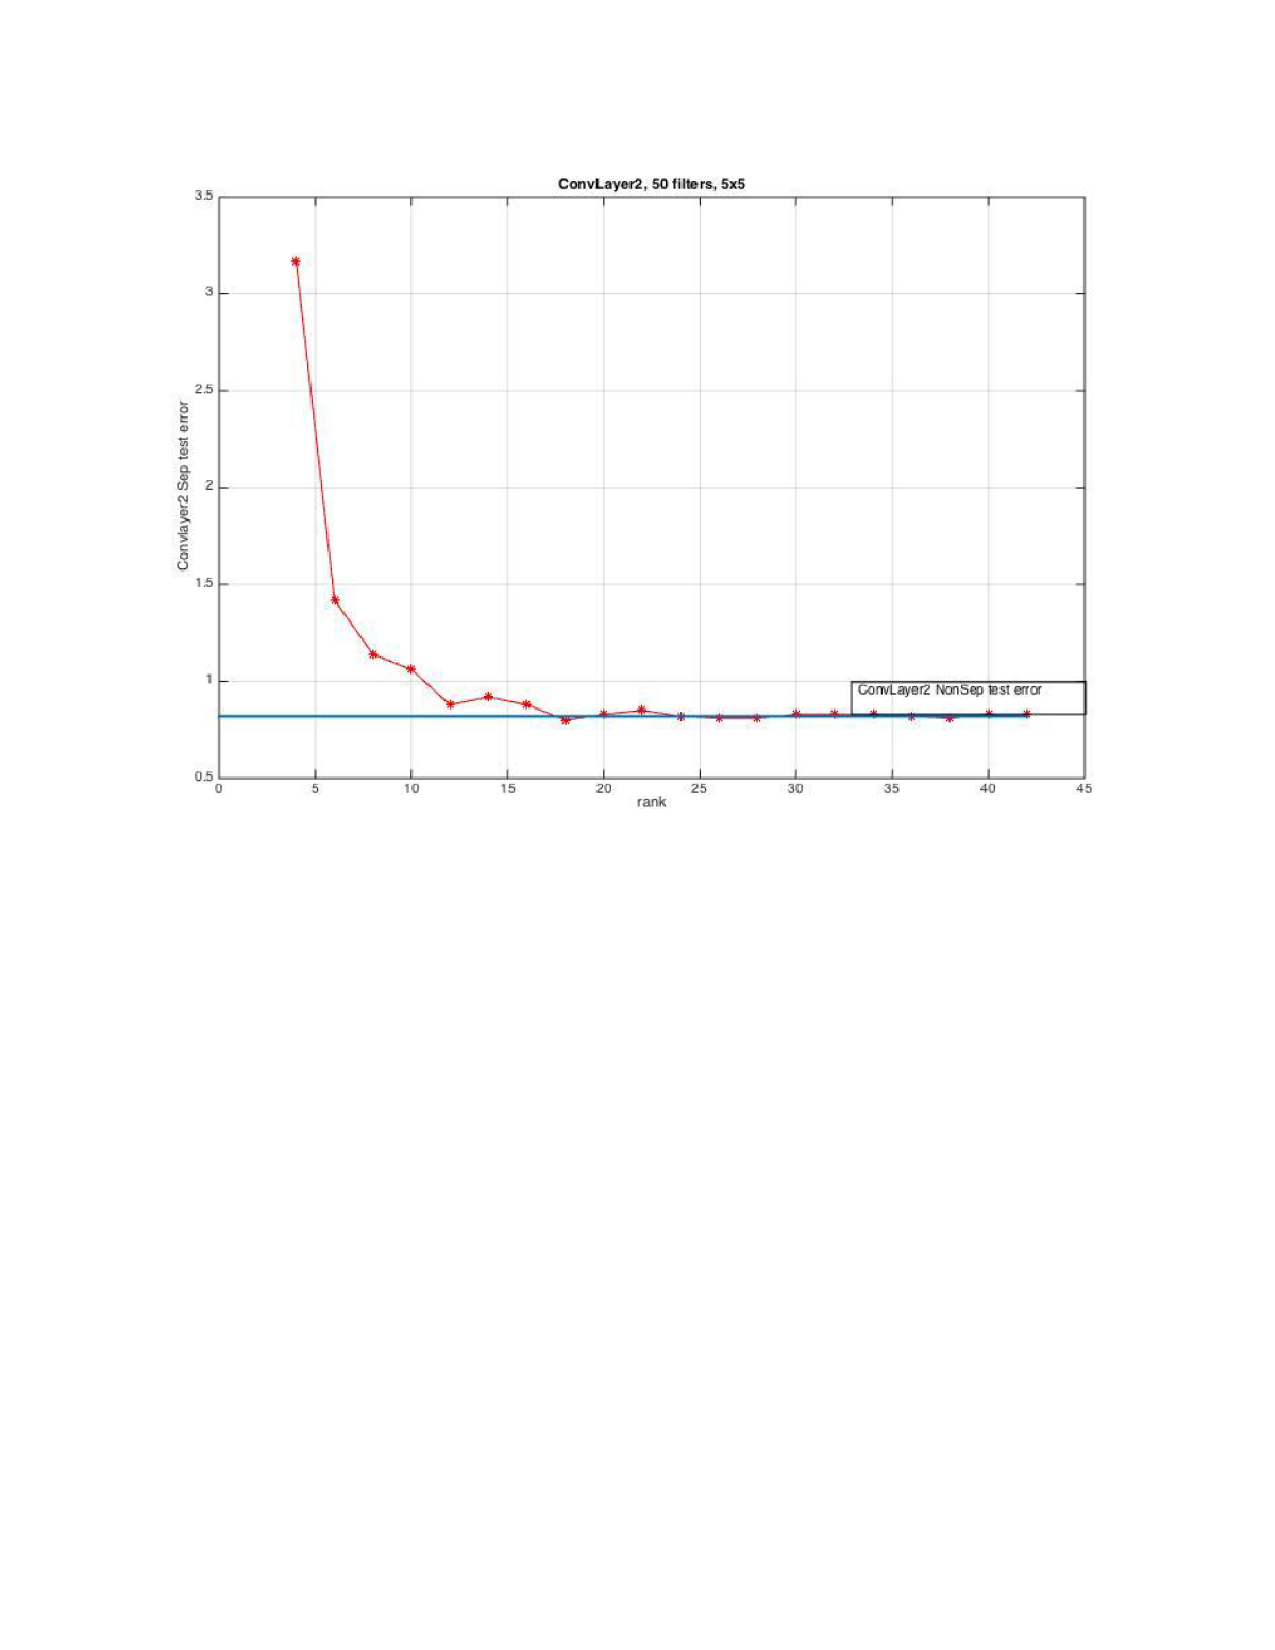
\includegraphics[width=\textwidth]{images/imagesCNN_page1.pdf}
    \caption{}
  \end{subfigure}
  \begin{subfigure}[b]{0.40\textwidth}
    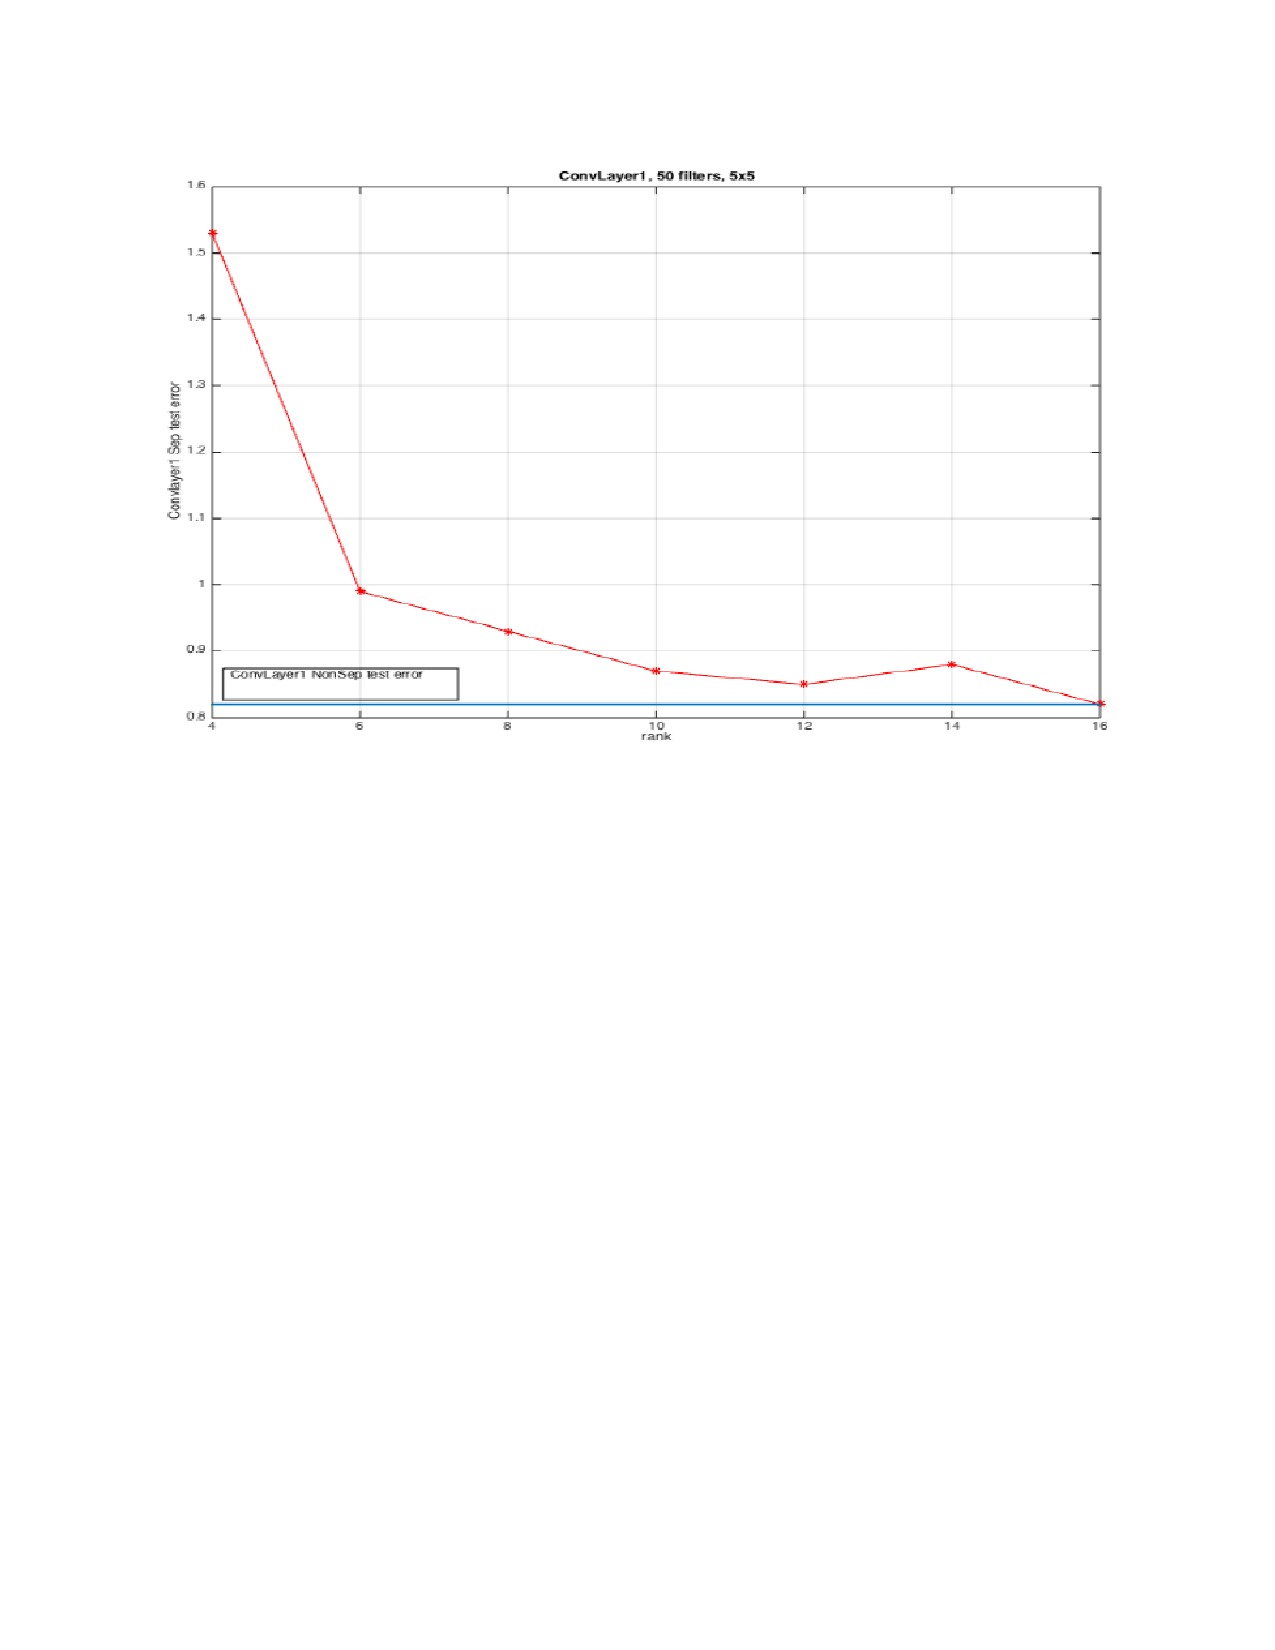
\includegraphics[width=\textwidth]{images/imagesCNN_page4.pdf}
    \caption{}
  \end{subfigure}
  \caption{Distribution of listening counts}
  \label{fig:user_artist_distribution}
\end{figure}

\begin{figure}[h]
  \centering
  \begin{subfigure}[b]{0.40\textwidth}
   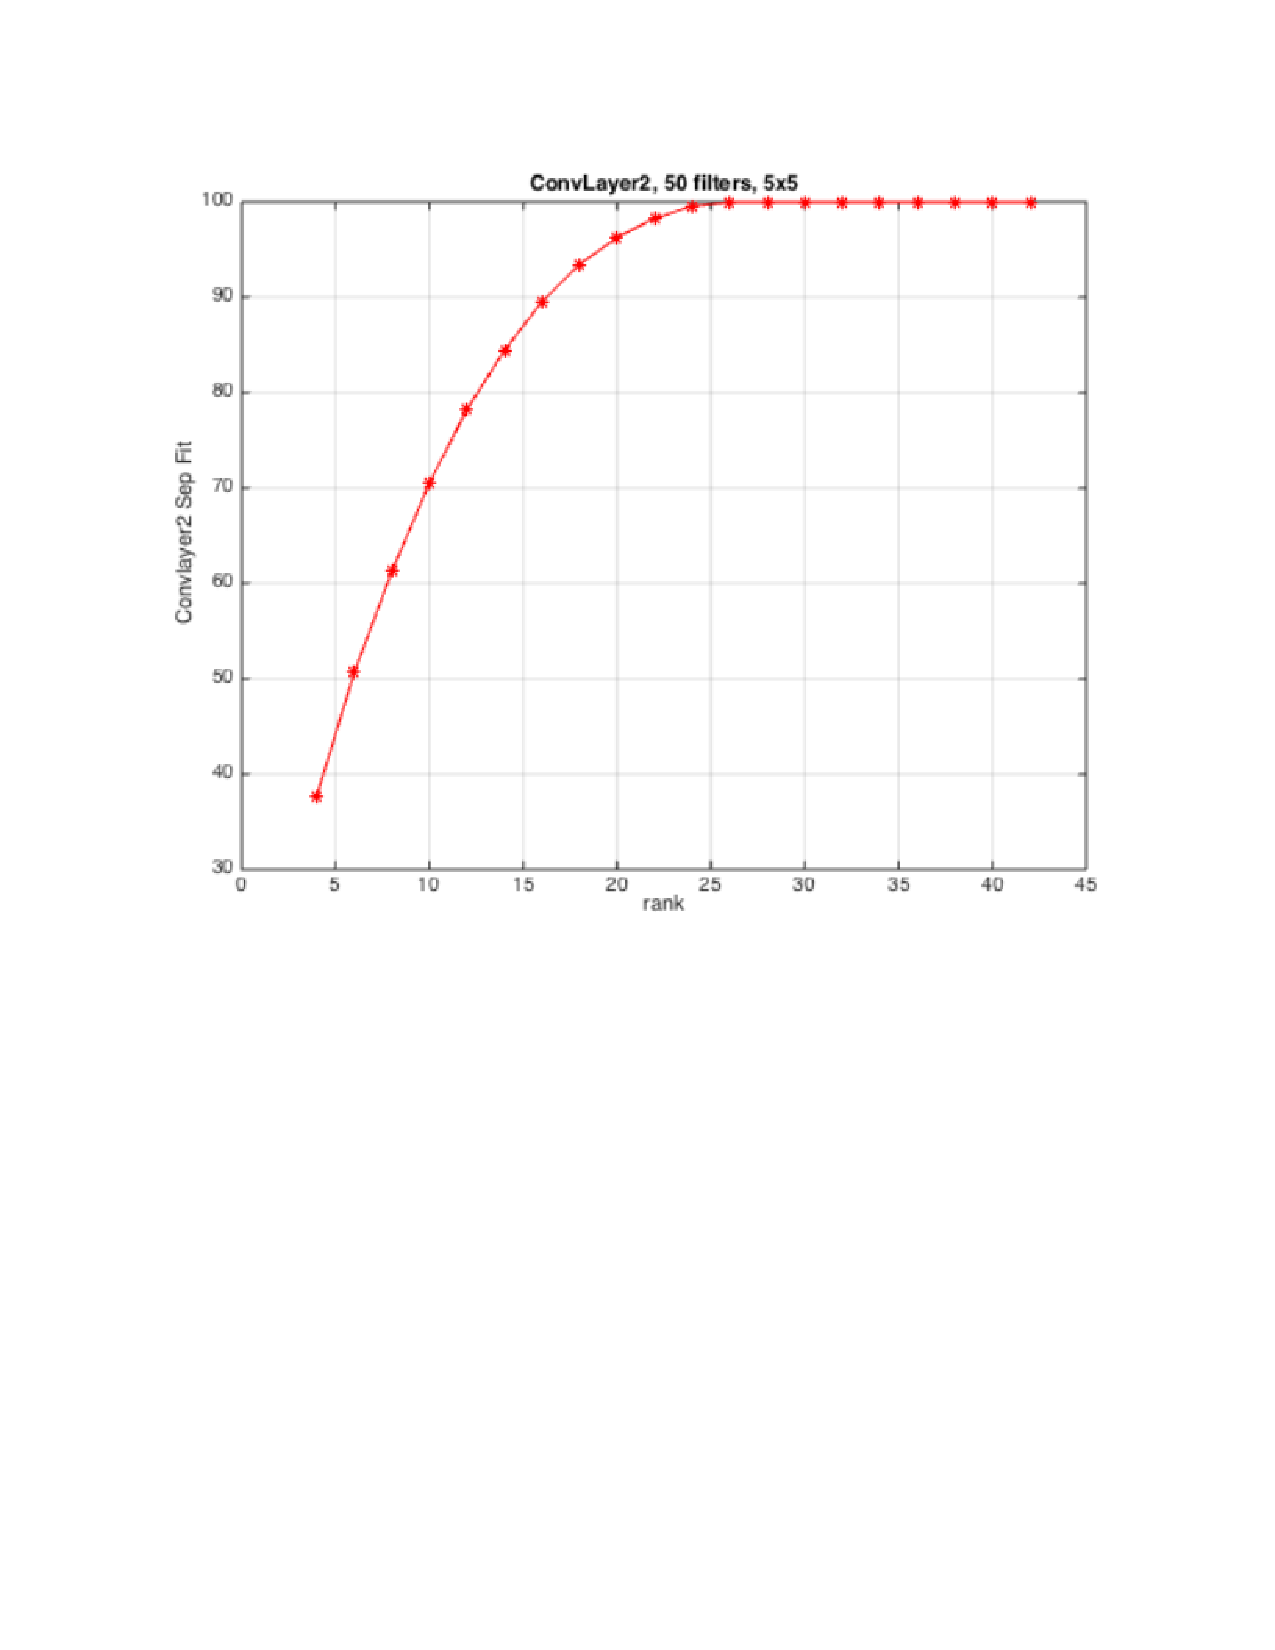
\includegraphics[width=\textwidth]{images/imagesCNN_page2.pdf}
    \caption{}
  \end{subfigure}
  \begin{subfigure}[b]{0.40\textwidth}
    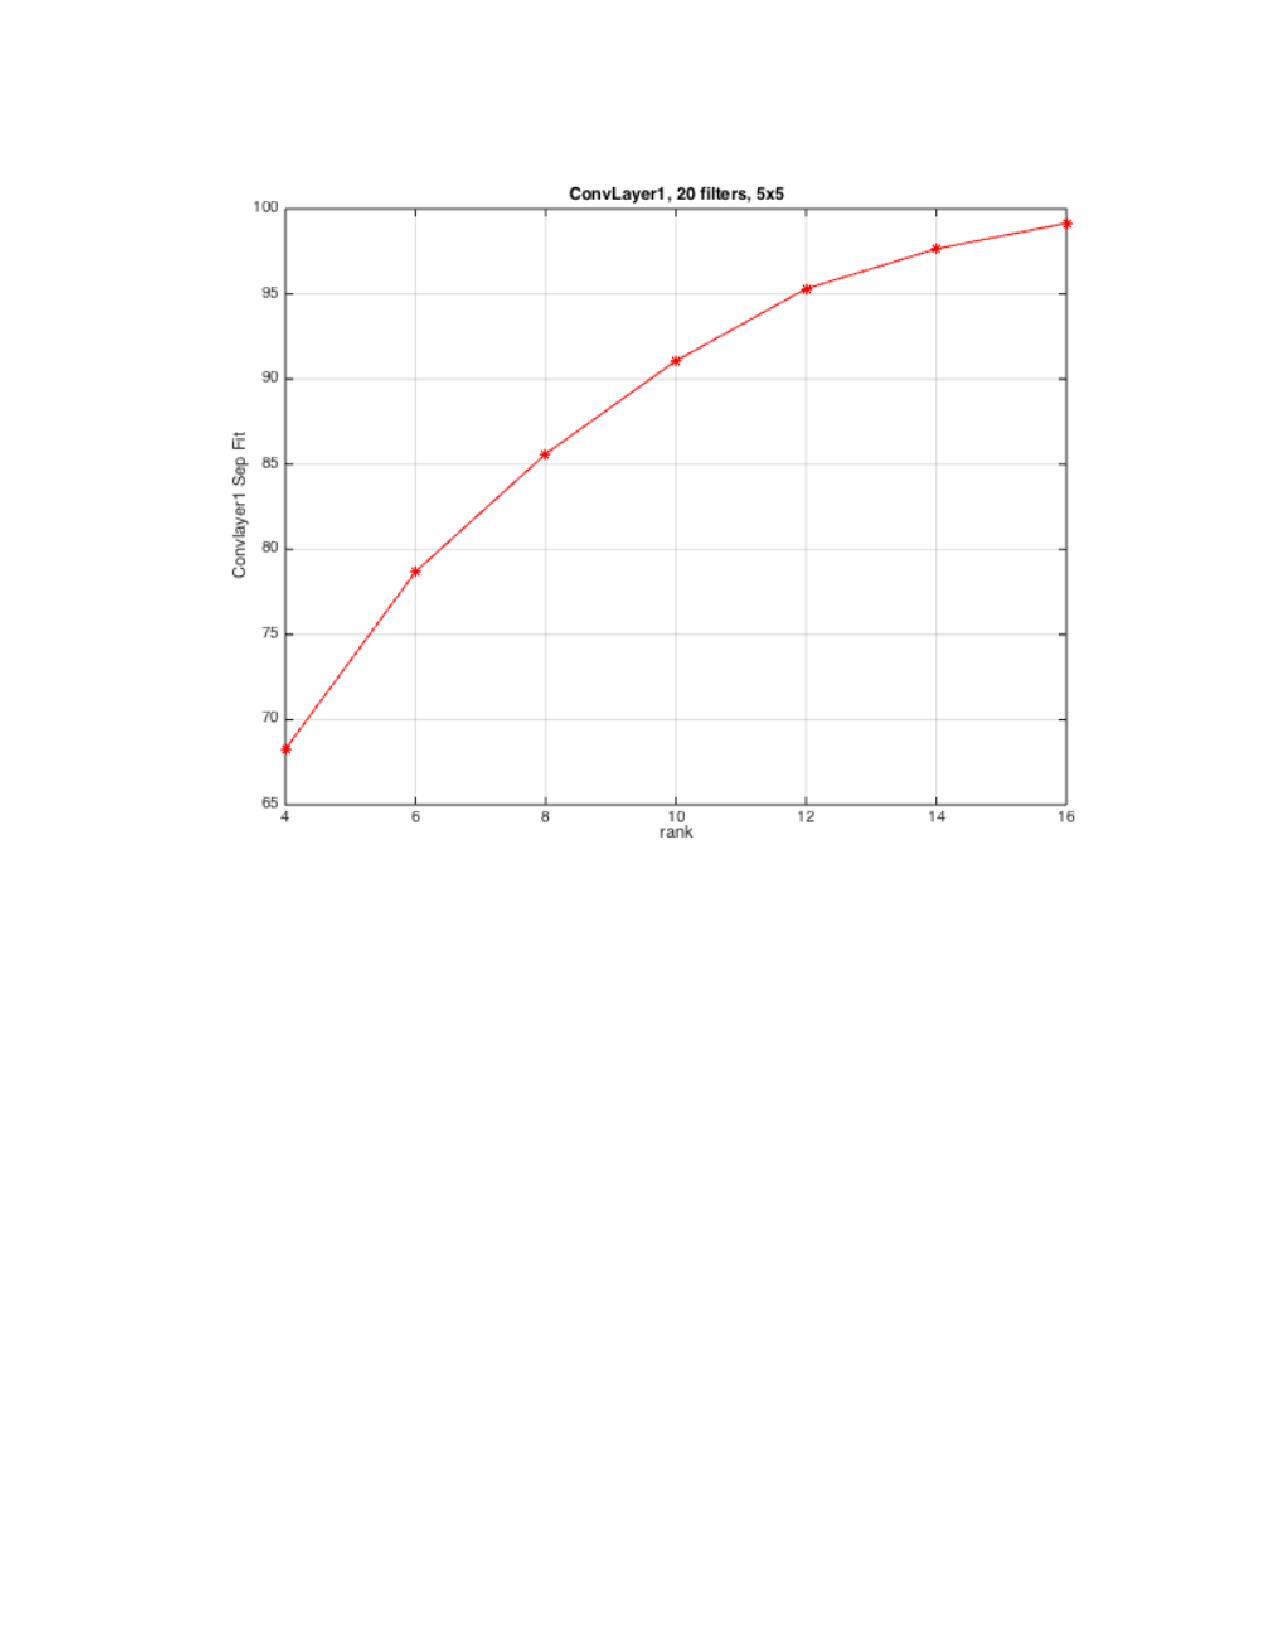
\includegraphics[width=\textwidth]{images/imagesCNN_page6.pdf}
    \caption{}
  \end{subfigure}
  \caption{Distribution of listening counts}
  \label{fig:user_artist_distribution}
\end{figure}

\begin{figure}[h]
  \centering
  \begin{subfigure}[b]{0.40\textwidth}
   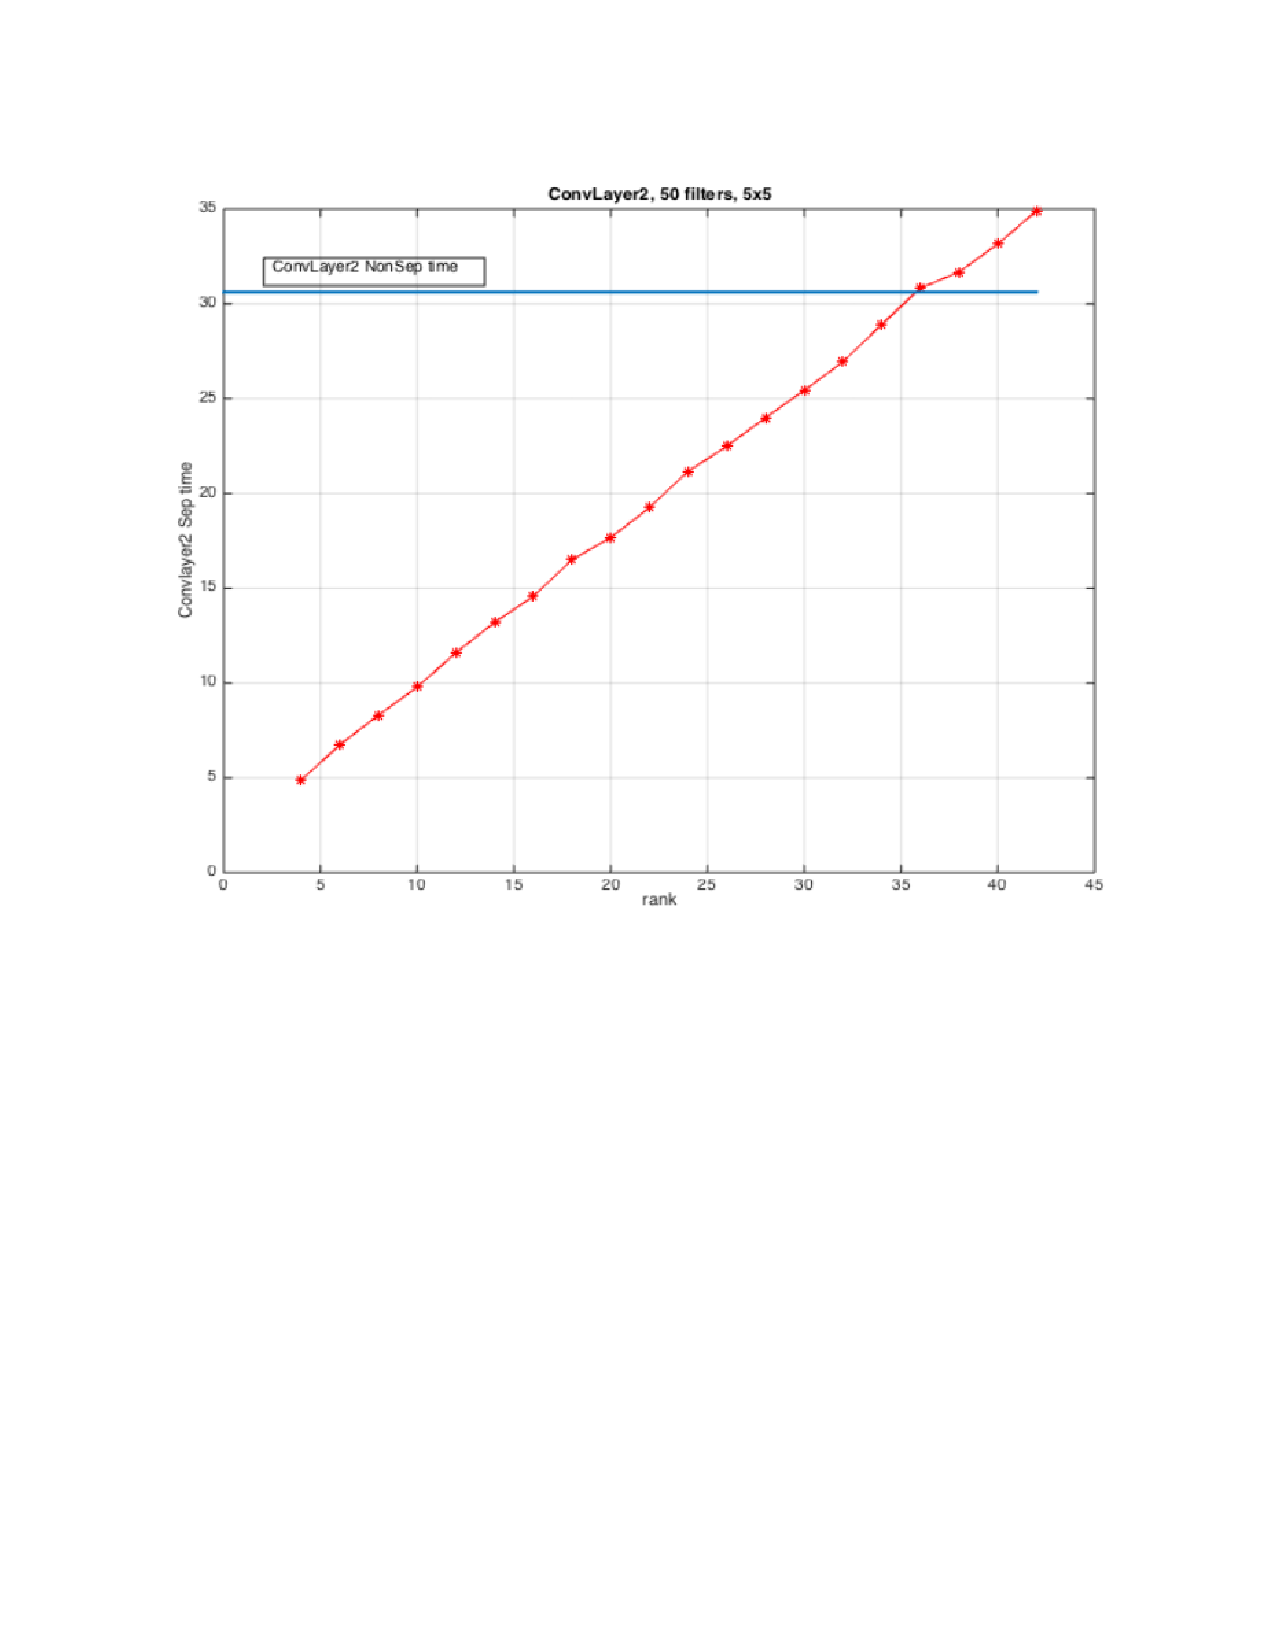
\includegraphics[width=\textwidth]{images/imagesCNN_page3.pdf}
    \caption{}
  \end{subfigure}
  \begin{subfigure}[b]{0.40\textwidth}
    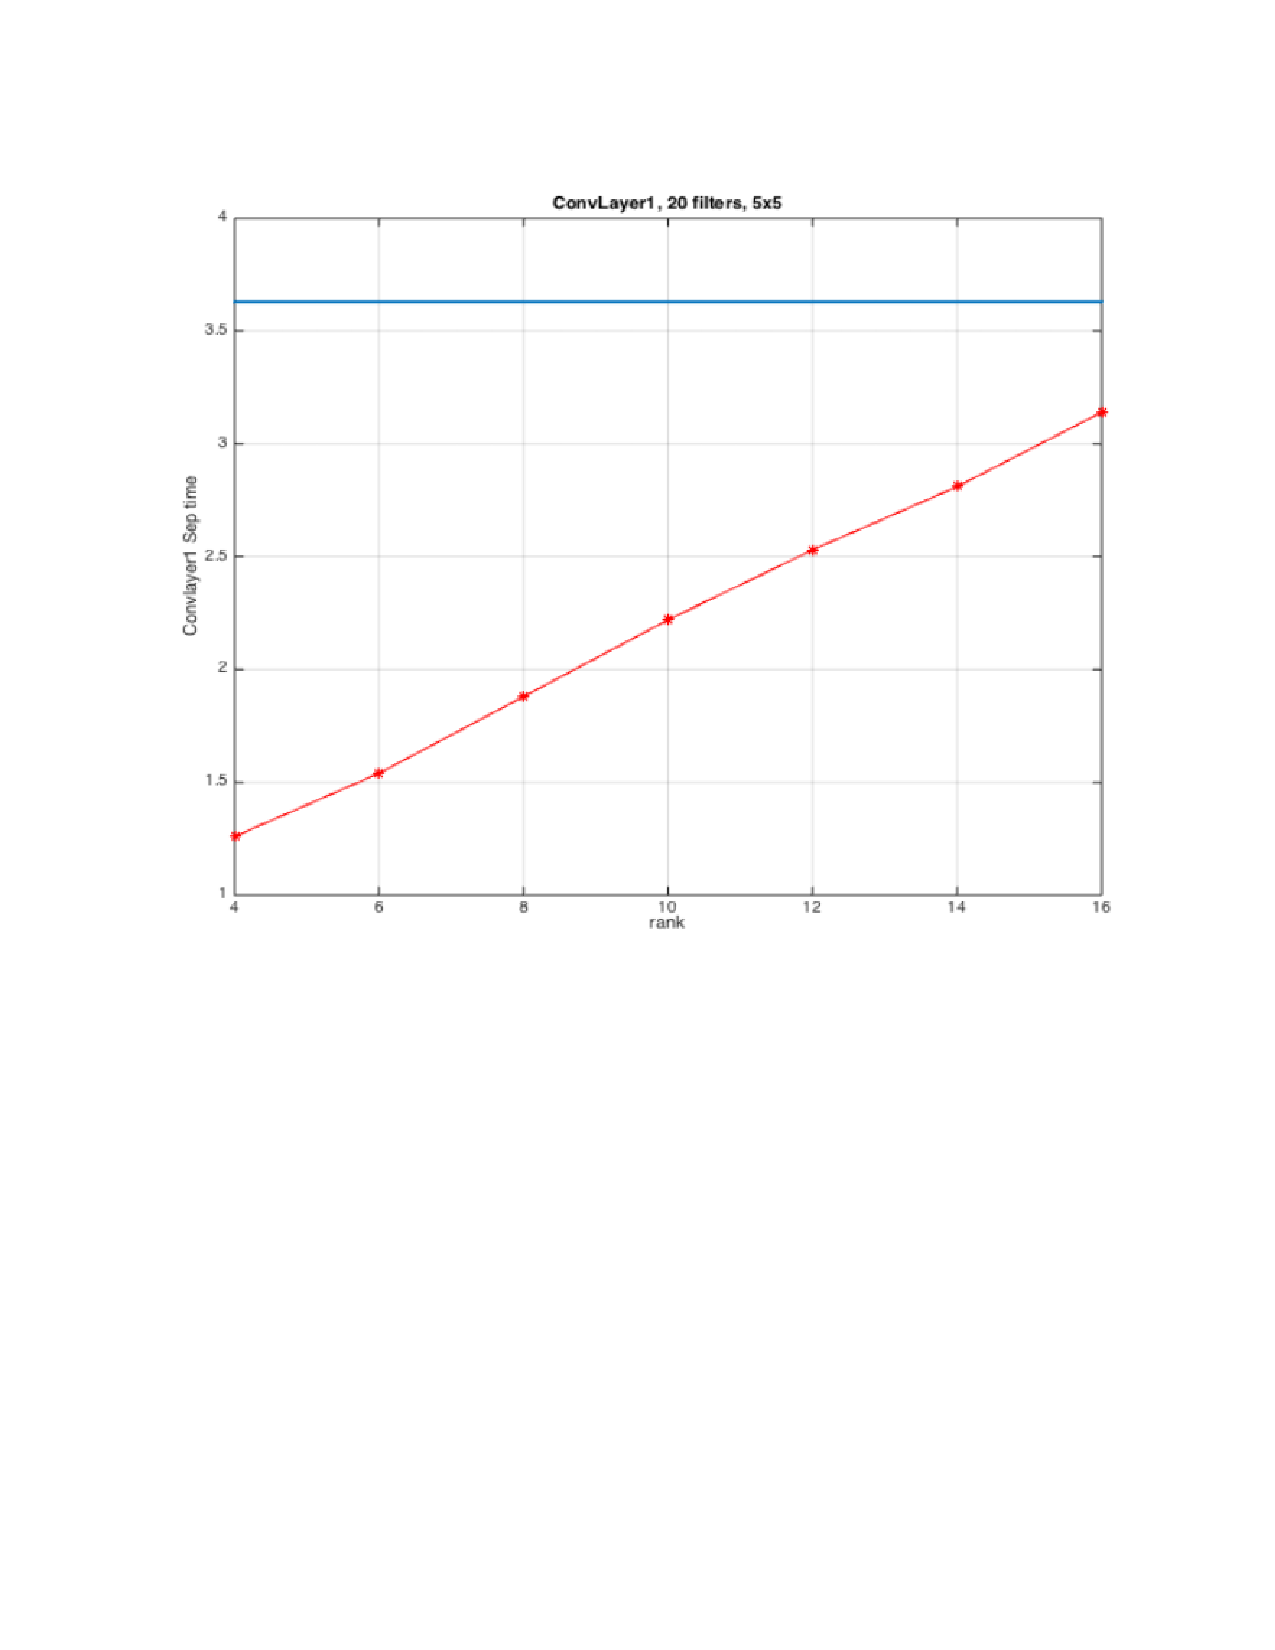
\includegraphics[width=\textwidth]{images/imagesCNN_page5.pdf}
    \caption{}
  \end{subfigure}
  \caption{Distribution of listening counts}
  \label{fig:user_artist_distribution}
\end{figure}

\subsubsection{Model 2}
\begin{table}
\centering
\begin{tabular}{@{}rlll@{}}\toprule
Layer & Type & Maps and neurons& Kernel size \\ \midrule
0 & input & 1 map of 28x28 &\\
1& convolutional & 20 maps of 24x24 & 9x9\\
2 & max pooling & 20 maps of 12x12 & 2x2 \\
3 & convolutional & 50 maps of 8x8& 9x9 \\
4 & max pooling & 50 maps of 4x4& 2x2 \\ 
5 & fully conntected& 500 & \\
6 & fully conntected & 2 neurons & \\ \bottomrule
\end{tabular}
\caption{Bigger CNN for MNIST set}
\end{table}


\subsection{Mitocondria}

\subsection{ImageNet}

\section{Conclusions}
Theoretical bounds of the separabe filters choice are proven.
Impreved recognition on mitocondria set.

\section*{Acknowledgments}
We would like to thank Simon Arosi that helped me a lot during this project giving me constant feedback.

\bibliography{citations}
\bibliographystyle{plain}

\end{document}

